\begin{tcolorbox}[colback=blue!5!white,colframe=blue!75!black,title=HMI - SCADA]
	Ambas tecnologías, HMI y SCADA, son utilizadas en conjunto en la industria de la automatización. SCADA proporciona funciones de supervisión, alarmas y control, mientras que HMI proporciona las herramientas que necesita para desarrollar imágenes que los operadores pueden usar para monitorear su proceso. El HMI se utiliza para monitorear o visualizar lo ejecutado por SCADA.
\end{tcolorbox}

\subsection{MBE}
\subsection{iFix}
\subsubsection{Guia}
\subsubsection{Programa}


Se realizó una interfaz humana maquina con los siguientes elementos:
\begin{itemize}
	\item boton de start(acá o en el tablero???)
	\item varias velocidades configuradas previamente
	\item inversión y señalización del mismo
	\item torque???
	\item HMI
	      \subitem Alarmas
	      \subitem Información en tiempo real
	      \subitem Histórico de datos
	      \subitem Control general del banco
\end{itemize}
\begin{figure}[htb]
	\centering
	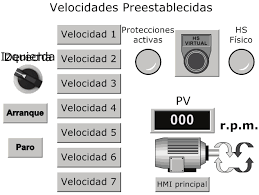
\includegraphics{HMIej.png}
	%\caption{Placa BME280}
	%\label{fig:BME280}
\end{figure}

\subsubsection{Alarmas- iHistorian}